\textbf{Hội tụ mạnh chùm tia bằng tứ cực từ}

Trong các máy gia tốc hạt, để hội tụ các chùm tia tích điện thì hệ các cặp tứ cực từ đặt lệch so với nhau góc $\SI{90}{^\circ}$ thường được sử dụng. Ở vùng trung tâm một tứ cực từ, vector điện trường $\Vec{B}$ có dạng gần đúng trong hệ tọa độ Decartes là (tuyến tính theo độ lệch trục):
\begin{equation*}
    \Vec{B} = g \left( y \hat{x} + x \hat{y} \right),
\end{equation*}
với $g$ là một hệ số phụ thuộc vào cấu trúc của tứ cực từ.

\begin{enumerate}
    \item \textbf{Tứ cực từ} \\
    Xét một mô hình đơn giản của tứ cực từ tạo bởi 4 lưỡng cực từ có moment lưỡng cực $p_m$ nằm ở 4 góc của một hình vuông có cạnh là $a \sqrt{2}$. Hai lưỡng cực từ chéo góc có chiều hướng về phía tâm và hai lưỡng cực từ chéo góc còn lại có hướng ngược chiều hướng tâm (như hình 1). Hãy tìm hệ số $g$ trong trường hợp này theo $p_m$, $a$ và hằng số từ $\mu_0$.
\begin{center}
\begin{minipage}{0.4\textwidth}
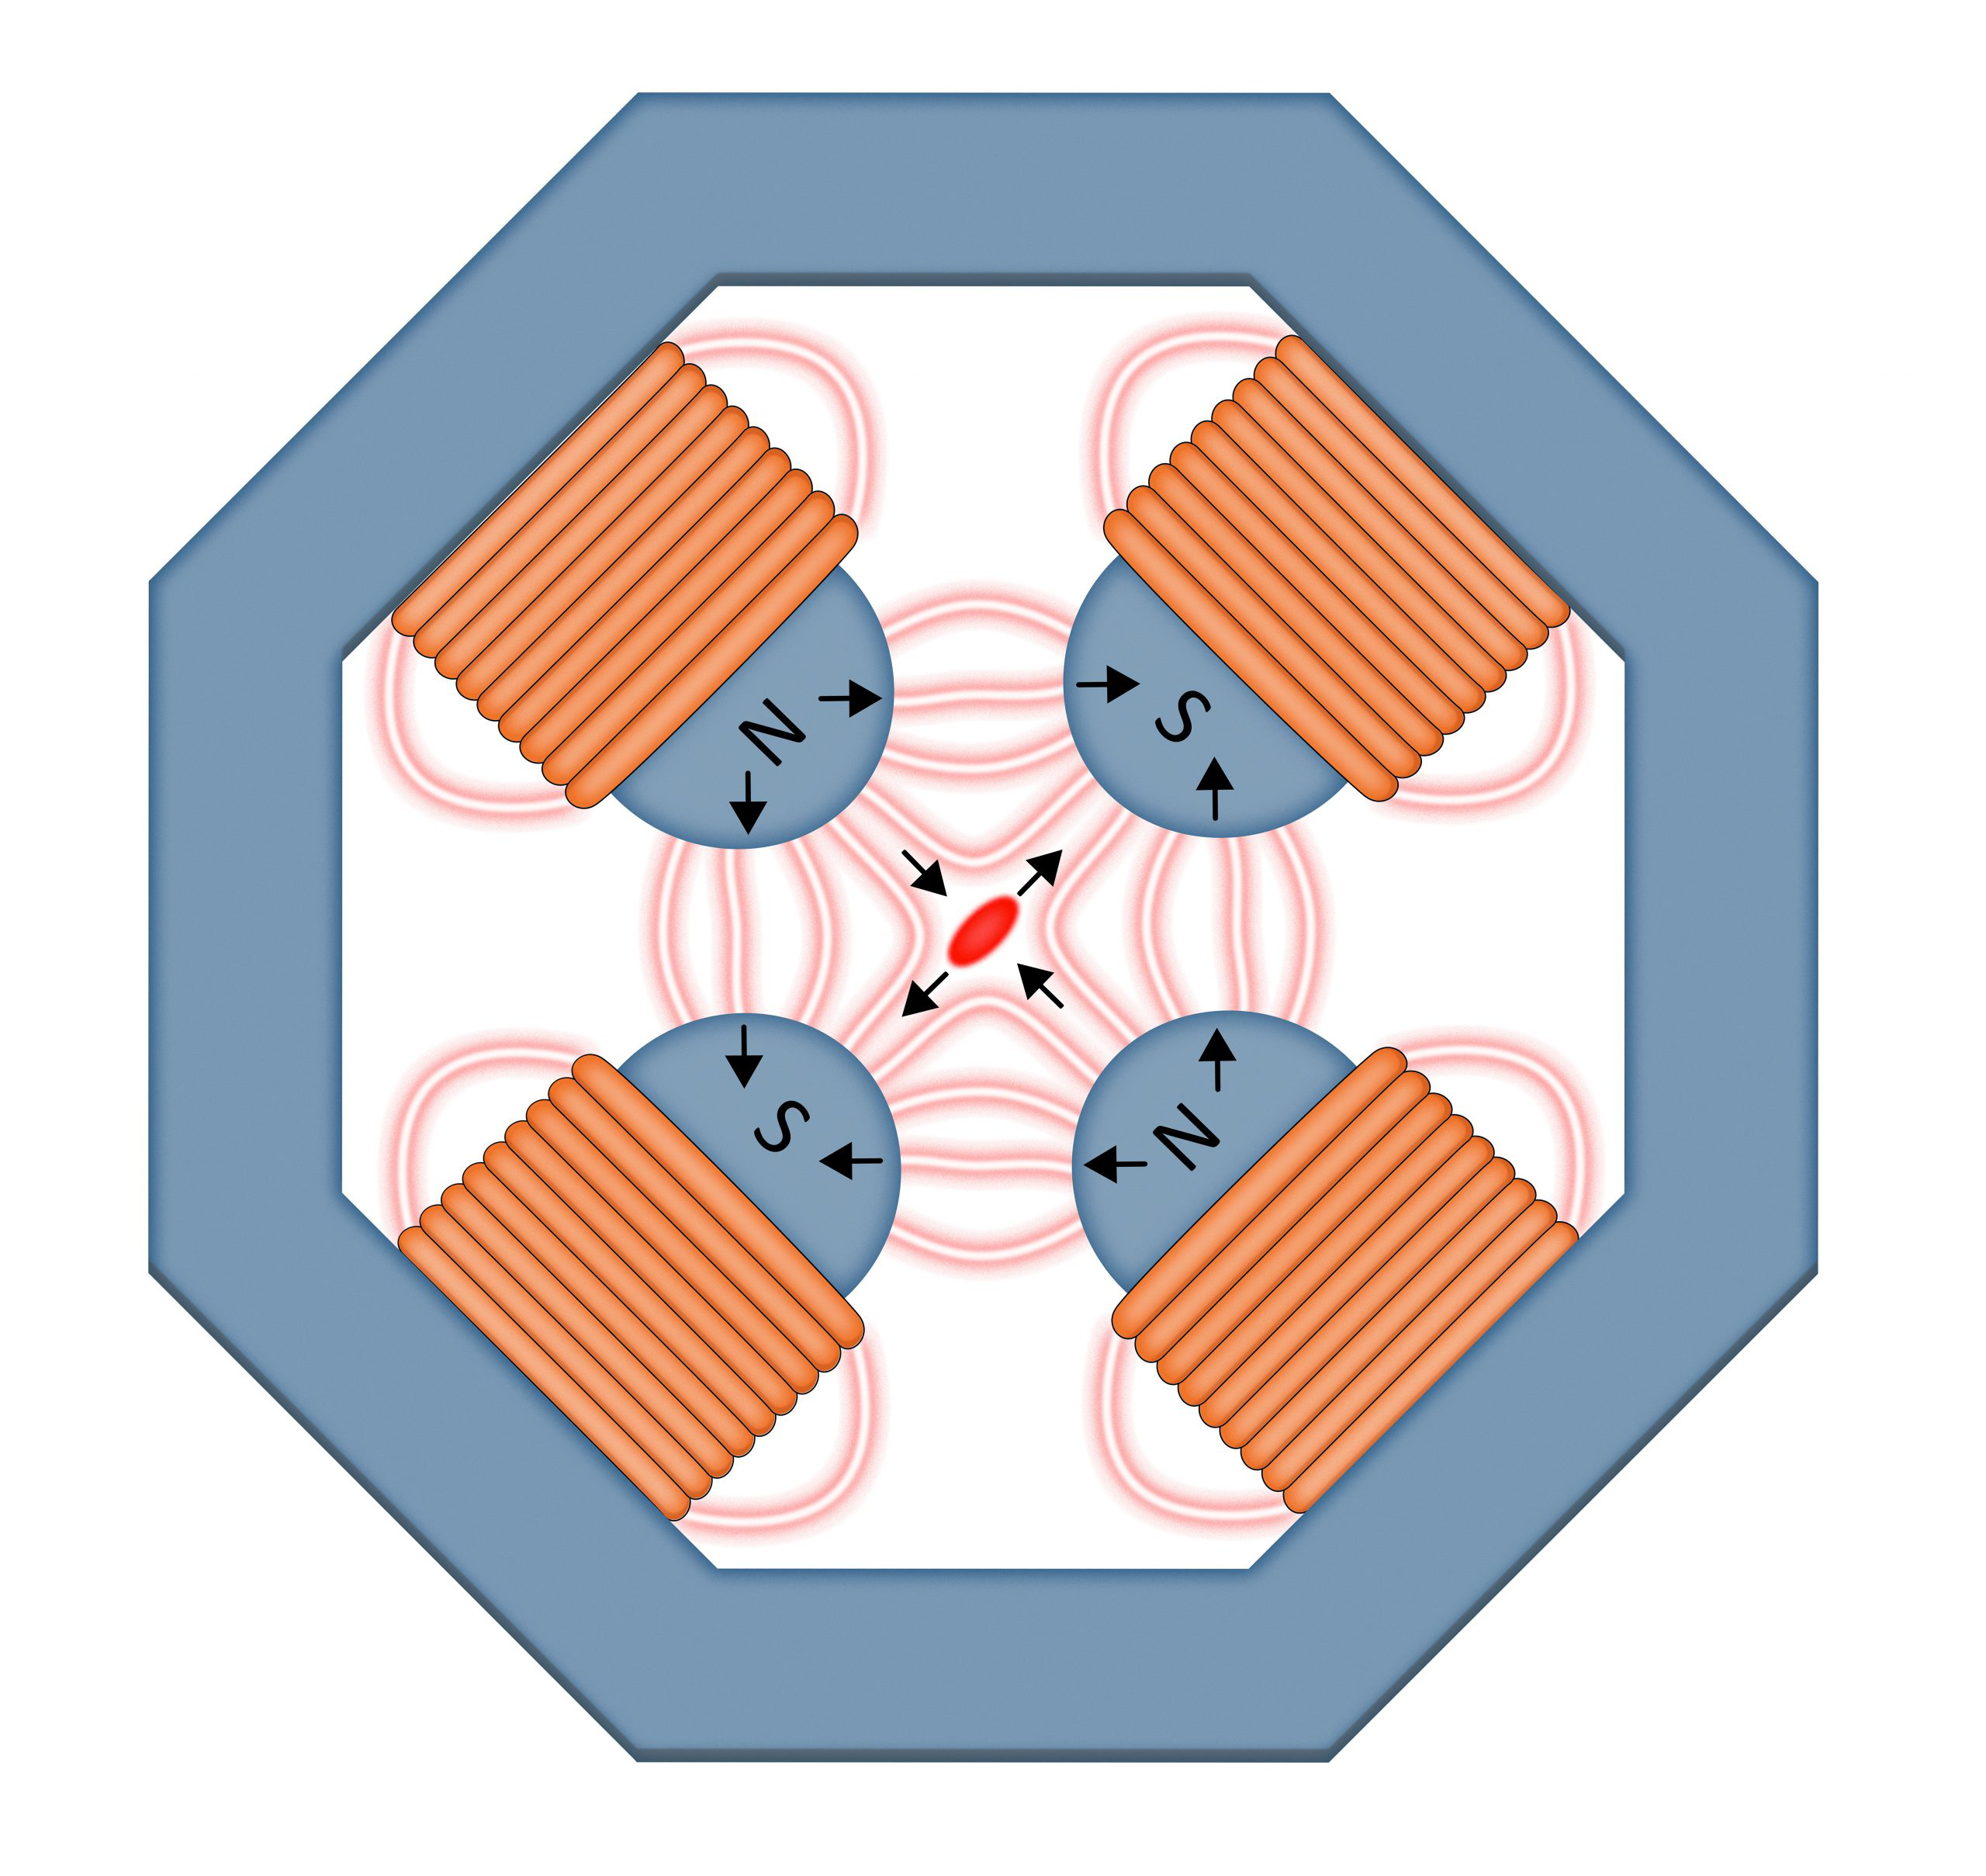
\includegraphics[width=0.9\textwidth]{Problem_18/quadrupoles.png}
\end{minipage}
\begin{minipage}{0.4\textwidth}
\centering
\begin{tikzpicture}[scale=0.7]
    \draw[-Stealth] (-4,0) to (4,0);
    \draw[-Stealth] (0,-4) to (0,4);
    \filldraw[color=black, fill=black, ultra thick] (0,0) circle (0.05);
    \draw (-0.3,0.3) node{$O$} (3.8,0) node[above]{$x$} (0,3.8) node[left]{$y$};
    \draw[dashed] (-3,-3) to (3,-3) to (3,3) to (-3,3) to (-3,-3);
    \draw[very thick, -Stealth] (-2.7,-2.7) to (-3.3,-3.3);
    \draw[very thick, -Stealth] (2.7,2.7) to (3.3,3.3);
    \draw[very thick, Stealth-] (2.7,-2.7) to (3.3,-3.3);
    \draw[very thick, Stealth-] (-2.7,2.7) to (-3.3,3.3);
\end{tikzpicture}
\end{minipage} \\
Hình 1: Mô hình tứ cực từ: (Bên trái) Trong thực tế; (Bên phải) Trong bài toán. 
\end{center}

    \item \textbf{Chuyển động của hạt qua một tứ cực từ} \\
    Một hạt điện tích q chuyển động với một động lượng $p$ lớn theo hướng gần như song song trục $Oz$ của một tứ cực từ. Để đơn giản, ta xem rằng hạt đi qua một tứ cực từ chỉ chịu ảnh hưởng của tứ cực từ trong một vùng dài $L$ [với $L \ll p/(qg)$] theo trục $Oz$ và từ trường trong vùng này có thể xem như không đổi theo tọa độ $z$. 
\begin{center}
\definecolor{9de0ad}{HTML}{9de0ad}
\definecolor{547980}{HTML}{547980}
\definecolor{594f4f}{HTML}{594f4f}
\begin{minipage}{0.4\textwidth}
\centering
\begin{tikzpicture}[scale=1]
    \draw[thick, fill=9de0ad] (-0.3,-2) rectangle (0.3,2);
    \draw[thick, 547980, -Stealth] (0.3,1) to (4,0);
    \draw[thick, 547980, -Stealth] (-2,1) to (0.3,1);
    \draw[thick, 547980, -Stealth] (0.3,-1) to (4,0);
    \draw[thick, 547980, -Stealth] (-2,-1) to (0.3,-1);
    \draw[thick, 594f4f, -Stealth] (-2.5,0) to (4.5,0);
    \draw (-0.3,0.5) node[left]{$x$} (2,0.05) node[below]{$f_x$} (4.3,0) node[above]{$z$} (0,1.5) node{$L$};
\end{tikzpicture}
\end{minipage}
\hspace{0.05\textwidth}
\begin{minipage}{0.4\textwidth}
\centering
\begin{tikzpicture}[scale=1]
    \draw[thick, fill=9de0ad] (-0.3,-2) rectangle (0.3,2);
    \draw[thick, 547980, dashed] (0.3,1) to (-4,0);
    \draw[thick, 547980, -Stealth] (0.3,1) to (1.16,1.2);
    \draw[thick, 547980, -Stealth] (-2,1) to (0.3,1);
    \draw[thick, 547980, dashed] (0.3,-1) to (-4,0);
    \draw[thick, 547980, -Stealth] (-2,-1) to (0.3,-1);
    \draw[thick, 547980, -Stealth] (0.3,-1) to (1.16,-1.2);
    \draw[thick, 594f4f, Stealth-] (2,0) to (-4.5,0);
    \draw (-0.3,0.5) node[left]{$y$} (-1.8,0.05) node[below]{$-f_y$} (1.8,0) node[above]{$z$} (0,1.5) node{$L$};
\end{tikzpicture}
\end{minipage} \vspace{3mm} \\
Hình 2: Quỹ đạo của hạt trong mặt phẳng $xOz$ (bên trái) và $yOz$ (bên phải).
\end{center}
    Theo định luật Earnshaw, trong trường tĩnh điện (và tương tự với từ trường) sẽ không tồn tại một vị trí cân bằng bền. Hiểu đơn giản trong trường hợp này, chúng ta có thể chỉ ra rằng nếu như chuyển động của hạt theo phương $x$ có một vị trí cân bằng bền để hạt dao động quanh thì vị trí cân bằng tương tự theo phương $y$ sẽ không phải vị trí cân bằng bền (và ngược lại). Như vậy, tứ cực từ giống như một thấu kính kỳ lạ, hội tụ đối với phương $x$ và phân kỳ đối với phương $y$ (như hình 2). Hãy tìm các tiêu cự $f_x$ và $f_y$ ứng với mỗi phương của thấu kính này theo $g$, $q$, $p$ và $L$.
    \item \textbf{Hội tụ chùm tia} \\
    Để chùm tia đi qua hệ hội tụ, người ta thường sử dụng các tứ cực từ thành từng cặp đặt lệch nhau $\SI{90}{^\circ}$ và cách nhau một khoảng $d$ (xem hình 3). Độ lớn các tiêu cự của các tứ cực từ là $f$. Hãy tìm tiêu cự tương đương qua toàn hệ $f'_x$ và $f'_y$ theo $f$ và $d$, chỉ ra điều kiện để chùm tia này hội tụ theo từng phương.
\end{enumerate}

\begin{center}
\hspace{0.05\textwidth}
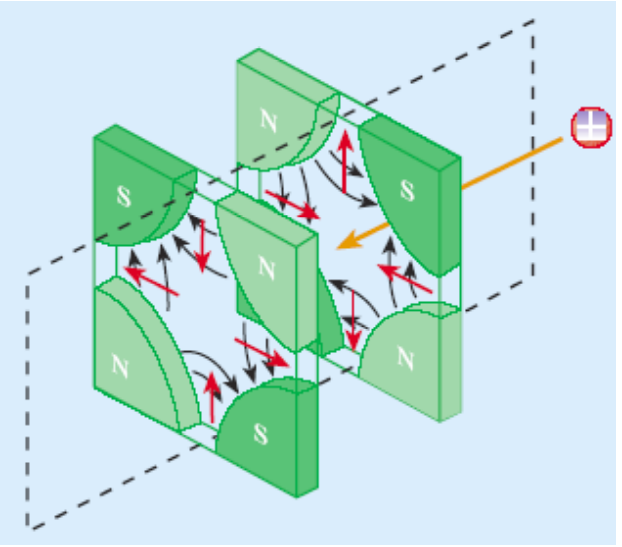
\includegraphics[width=0.38\textwidth]{Problem_18/two_quadrapole.png}
% \hspace{0.05\textwidth}
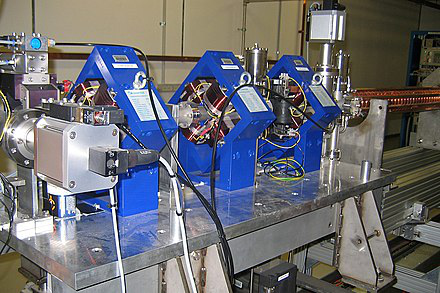
\includegraphics[width=0.5\textwidth]{Problem_18/Synchrotron_Quadrupole.png} \\
    Hình 3: Cặp tứ cực từ (bên trái) và máy gia tốc hạt hội tụ mạnh sử dụng các tứ cực từ (bên phải).
\end{center}

\begin{flushright}
    (Biên soạn bởi Bourbaki và Log)
\end{flushright}